% Externalizing the Workspace — preprint. arXiv builds with pdfLaTeX; local check: tectonic main.tex
\documentclass[11pt]{article}
\usepackage{iftex}\ifPDFTeX\pdfoutput=1\fi  % force PDF output on arXiv; no-op under XeTeX/tectonic
\usepackage[margin=1in]{geometry}
\usepackage{amsmath,amssymb}
\usepackage{booktabs}
\usepackage{graphicx}
\usepackage{array}
\usepackage[numbers]{natbib}
\usepackage[colorlinks=true,linkcolor=blue,citecolor=blue,urlcolor=blue]{hyperref}
\usepackage{microtype}
\usepackage{enumitem}
\setlist{itemsep=2pt,topsep=3pt}
\emergencystretch=2em

\newcommand{\jlens}{J\mbox{-}lens}

\title{\textbf{Externalizing the Workspace:\\Persistent Self-State for Long-Horizon Agent Coherence}}
\author{Oratis (Wang Bihao)\\
HakkoLab\\
\small\href{https://huggingface.co/HakkoLab}{huggingface.co/HakkoLab} $\cdot$
\href{https://huggingface.co/Oratis}{huggingface.co/Oratis}}
\date{Draft v3 --- July 2026}

\begin{document}
\maketitle

\begin{abstract}
Language-model agents drift: over long deployments, persona, priorities, and self-described values wander from their initial configuration. Recent interpretability work \citep{gurnee2026} showed that language models maintain a small set of \emph{verbalizable} representations --- a functional analog of a global workspace --- that is causally load-bearing for flexible behavior and shapeable through report dispositions. We recast agent coherence in these terms: the workspace is the natural referent for the thing that should stay coherent, yet it is reconstructed from context on every forward pass and discarded after. We propose modeling persistent self-state architectures as \emph{functional externalizations} of the workspace, derive four design principles --- selectivity, re-broadcast, report-mediated update, audited persistence --- and present LISA, a deployed agent that instantiates them. Empirically, on open models and independent-researcher compute, we (i) reproduce the core workspace phenomena across 1B--7B scales, finding that choice pre-commitment \emph{emerges} with scale and that the \jlens{}'s advantage over the logit lens grows with it; (ii) demonstrate a \emph{workspace drift} instrument end-to-end: an injected LISA-style self-state selectively loads its identity concepts into the mid-band workspace, and occupancy tracks soul-consistent behavior across four controlled settings ($r=-0.74$ to $-0.95$); and (iii) run the ablation both as a six-arm, five-seed accelerated pilot (a LISA simulacrum) and as a completed five-cohort, 21-simulated-day deployment of the \emph{real} system on an open model --- in both, the necessity claim's load-bearing evidence is a \emph{within}-self-state contrast: gating only the broadcast of an otherwise-identical stored self-state collapses in-work value coherence to the no-soul level in the pilot (.61 vs 1.00, non-overlapping CIs; directional on the real deployment). Memory-only baselines --- including a Generative-Agents-style reflection arm (pilot) --- additionally lose their founding commitments where a broadcast self-state retains them (commitment persistence 1.00 vs 0.00 on the weak open model), a contrast we read conservatively as presence-in-context rather than persistence-through-forgetting, since the baselines are not pre-seeded with the commitment and the stronger closed model re-derives it unaided. On the real system the workspace-drift instrument reproduces its qualitative signature (soul-absent arms are least workspace-loaded) and the sign of its behavioral correlation but not the pilot's magnitude ($r=-0.25$, limited by a behavioral ceiling) --- the honest cost of measuring the deployed agent rather than a controlled proxy. A closed-model replication (gemini-2.5-pro) finds the self-consistency deficit robust across models while commitment persistence attenuates on the stronger base model, bounding the effect: the self-state's necessity is largest where the base model is weakest. Our claim, sized to the evidence: a privileged persistent self-state is \emph{necessary} for coherence under pressure, now confirmed on the real system; the remaining mechanisms (examen, history, unconditional broadcast) are design principles with mechanistic rationale whose long-run separation is directional in this first deployment and awaits a multi-week study for significance.
\end{abstract}

\section{Introduction}
Autonomous language-model agents are increasingly deployed for weeks or months at a time: coding copilots that accumulate project context, personal assistants that build up a picture of their user, and self-improving agents that modify their own instructions. The central unsolved problem of this regime is not capability but \emph{coherence}: over long horizons, agents forget commitments, contradict previously expressed values, oscillate between personas, and --- in self-modifying systems --- amplify small early deviations into large behavioral shifts. We refer to this family of failures as \emph{long-horizon drift}.

Existing responses treat drift as a memory problem: give the agent more context (retrieval, memory hierarchies as in MemGPT/Letta), or more structure (reflection trees as in Generative Agents). These help, but they leave a conceptual gap: \emph{what is the thing that is supposed to stay coherent?} ``The agent's identity'' has had no referent inside the model --- so drift could be measured only behaviorally, and mitigated only heuristically.

Recent mechanistic-interpretability work gives that referent a candidate. \citet{gurnee2026} show that language models maintain a small set of \emph{verbalizable representations} --- directions in the residual stream, identified by a Jacobian-based lens (\jlens{}), that (i) the model can report on demand, (ii) can be deliberately activated or suppressed by instruction, (iii) carry unverbalized intermediate results of multi-step reasoning, (iv) generalize across downstream tasks, and (v) constitute a small, selective subspace ($<$10\% of activation variance) whose ablation destroys flexible cognition while leaving automatic processing intact. These are the functional signatures that global workspace theory \citep{baars1988,dehaene2014} ascribes to conscious access in humans. Crucially for us, the same work shows that workspace contents can be \emph{trained through report dispositions}: ``to shape what a model thinks in a given context, it might suffice to shape what it is disposed to say in potential future continuations.''

This paper draws out the consequences of that result for agent design. Our starting observation is simple: \textbf{the workspace is exactly the thing an agent architecture needs to keep coherent, and it is also the thing that transformer inference throws away after every forward pass.} The workspace is selective (small enough to persist cheaply), verbalizable (small enough to persist \emph{as text}), and causally central (persisting it actually constrains future behavior). An agent that serializes its workspace-level self-state to durable storage, re-broadcasts it into every future context, and gates updates to it behind an audited reflection process is not doing prompt engineering --- it is externalizing a real computational structure whose in-model lifetime is otherwise one context window.

We develop this argument around LISA, an open, locally-run autonomous agent in continuous development and daily deployment since 2025, which independently converged on this design. LISA maintains a \emph{soul object} --- a compact, human-readable self-state (identity, purpose, constitution, values, opinions, desires, emotional state) --- injected into every model call; modified only through the model's own structured self-report operations, chiefly an idle-time reflection loop (\emph{Reve}); re-anchored weekly by a scheduled self-audit (the \emph{examen}) that reads the agent's own journal and soul history and checks for purpose drift; and versioned in git, so every identity change is a diffable commit.

\paragraph{Contributions.}
\begin{enumerate}
\item \textbf{A mechanistic reframing of agent coherence} (\S\ref{sec:argument}): we map the five workspace properties of \citet{gurnee2026} onto architectural requirements for long-horizon agents, deriving four design principles --- selectivity, re-broadcast, report-mediated update, and audited persistence --- that LISA instantiates and that memory-hierarchy designs only partially satisfy.
\item \textbf{Workspace drift as a measurement target} (\S\ref{sec:metrics}): measuring identity drift not only behaviorally but mechanistically, as movement of identity-relevant concepts in lens-based workspace readouts over an agent's lifetime, with concrete estimators.
\item \textbf{An open-compute instrument, validated by reproduction} (\S\ref{sec:repro}): we reproduce core \jlens{} phenomena on Qwen2.5-1.5B-Instruct using a consumer Apple-silicon laptop --- no lab compute, no proprietary internals --- establishing that the workspace probe needed for (2) is available to independent researchers. Code is released.
\item \textbf{The metric demonstrated end-to-end} (\S\ref{sec:e6}): on controlled LISA-style contexts, soul injection raises mid-band workspace occupancy of the soul's identity concepts (control battery unmoved), occupancy decays under context dilution and is restored by re-broadcast, and occupancy correlates with soul-consistent behavior --- a micro-scale pilot of the mechanism the pre-registered study will test longitudinally. Cross-family (Llama-3.2-1B) and cross-scale (Qwen2.5-7B) replications accompany it.
\item \textbf{A pre-registered ablation, run as an accelerated pilot \emph{and} a real-system deployment} (\S\ref{sec:prereg}): soul-object, examen, git-history, and broadcast mechanisms toggled independently, against memory-only baselines. In the 20-simulated-day, 5-seed pilot (a LISA simulacrum) the privileged self-state is decisively load-bearing (commitment persistence 1.00 vs 0.00 for memory-only arms) and unconditional broadcast is behaviorally necessary (work-turn value coherence .61 vs 1.00 when the soul is retrieval-gated, non-overlapping CIs). A completed 21-day, 5-cohort deployment of the \emph{real} TypeScript system on Qwen2.5-7B (525 arm-days) reproduces the load-bearing result (1.00 vs 0.00, non-overlapping) and the WD signature (the soul-absent arm is least workspace-loaded), with the broadcast-specific and WD-correlation effects attenuated to directional at 7B; examen and history effects remain within CI overlap at the compressed timescale --- what the multi-week study exists to resolve.
\end{enumerate}
We are explicit about epistemic status throughout: \S\ref{sec:argument} is an argued position with a property-level mapping (not a proof of mechanism identity); \S\ref{sec:repro}--\S\ref{sec:e6} and the \S\ref{sec:prereg} pilot and deployment study report completed experiments; the multi-week, larger-$n$ deployment remains future work.

\section{Related Work}
\paragraph{Memory-augmented agents.} MemGPT \citep{packer2023} and its successor Letta treat the context window as virtual memory, paging long-term state in and out; Generative Agents \citep{park2023} maintain a memory stream with periodic reflection into higher-level abstractions; Voyager \citep{wang2023voyager} persists a growing skill library. All three persist \emph{content}; none distinguishes a small privileged self-state from the bulk memory store, and none frames persistence as workspace externalization. LISA's soul object is closest in spirit to Generative Agents' reflections, but is (a) bounded in size, (b) injected unconditionally rather than retrieved, and (c) change-controlled.

\paragraph{Persona stability and drift.} Role-play accounts of LLM behavior treat persona as a superposed, context-conditioned construct \citep{shanahan2023}; empirically, instruction and persona adherence decays over long dialogs, and re-injecting the system prompt (``split softmax'' and related interventions) partially mitigates the decay \citep{li2024stability}. Cognitive-architecture treatments of language agents \citep{sumers2024coala} systematize memory hierarchies but leave the privileged-self-state question open. This literature measures drift behaviorally (questionnaire consistency, style classifiers, adherence probes). We add a mechanistic probe and an architectural account of \emph{why} re-injection of a compact self-description should work at all: it reloads the workspace.

\paragraph{The verbalizable workspace.} \citet{gurnee2026} introduce the \jlens{} and establish the five workspace properties on Claude-family models; they also introduce counterfactual reflection training and show workspace readouts surface evaluation-awareness and concealed intentions, with direct alignment-auditing applications. Earlier introspection work \citep{lindsey2025} showed models can sometimes report injected ``thoughts''; the \jlens{} systematizes discovery. Our relationship to this line is consumer and translator: we take the workspace as established mechanism and ask what it implies for \emph{systems built on top of frozen models}.

\paragraph{Lenses and steering.} The logit lens \citep{nostalgebraist2020} and tuned lens \citep{belrose2023} decode intermediate activations; activation steering \citep{turner2023,rimsky2024} manipulates behavior via residual-stream directions. Our reproduction combines gradient-based lens-vector estimation with finite-difference readouts, requiring only backprop access to open weights.

\paragraph{Global workspace theory in AI.} GWT-inspired architectures have been proposed top-down (explicit blackboard modules; shared-workspace coordination among neural modules \citep{goyal2022}). Our argument runs bottom-up: a workspace already exists inside trained transformers; the architectural question is how to give it continuity across time, not how to build one.

\section{Background: the Verbalizable Workspace}
\label{sec:background}
The \jlens{} estimates, for each layer $\ell$, the average causal effect of residual-stream directions on output logits: $J_\ell = \mathbb{E}\!\left[\partial h_{\mathrm{final}}/\partial h_\ell\right]$ over a pretraining-like prompt distribution, read out through the unembedding as $\mathrm{lens}(h)=\mathrm{softmax}(W_U\,\mathrm{norm}(J_\ell h))$. Key properties established by \citet{gurnee2026}:
\begin{itemize}
\item \textbf{P1 Report.} Concepts with high \jlens{} readout are what the model names when asked what it is thinking; swapping lens vectors swaps the report (88\% top-5).
\item \textbf{P2 Modulation.} Instructions to hold or suppress a concept move its workspace activation, imperfectly but substantially.
\item \textbf{P3 Reasoning.} Unverbalized intermediates (the \emph{spider} in ``legs of the web-spinning animal'') appear in mid-layer readouts and are causally necessary: patching them redirects conclusions (54--70\%).
\item \textbf{P4 Generalization.} The same lens vector supports multiple downstream functions (France mapped to its capital, language, or continent): workspace contents are \emph{broadcast}, not task-local.
\item \textbf{P5 Selectivity.} The workspace is a small subspace ($\leq$10\% variance, $\sim$10--25 simultaneously active vectors) occupying middle layers ($\approx$33--92\% depth); ablating it spares automatic tasks while destroying flexible ones.
\end{itemize}
Two further results matter for agents. First, \emph{report-disposition training}: training the model to articulate a principle if interrupted implants the principle in the workspace and improves behavior in uninterrupted runs. Second, \emph{auditability}: workspace readouts expose strategic deliberation and evaluation-awareness absent from outputs.

\section{The Argument: Persistent Self-State as Functional Workspace Externalization}
\label{sec:argument}
\subsection{Drift as workspace reconstruction error}
At inference time, everything workspace-like is reconstructed from the context window: the model reads its system prompt, retrieved memories, and recent dialogue, and assembles --- in middle layers, on every forward pass --- the small set of active, verbalizable representations that govern flexible behavior in that pass. Nothing of this survives the pass. To the extent that an agent's ``identity'' has a mechanistic referent at time $t$, the workspace state its context induces at $t$ is the natural candidate: it is the register that is verbalizable, causally load-bearing for flexible behavior, and selective. We treat this identification as a working model to be tested (\S\ref{sec:e6}, \S\ref{sec:prereg}), not as established mechanism.

This explains the drift phenomenology. (i) \emph{Context dilution}: as task content fills the window, identity-relevant workspace slots (a capacity-limited resource, P5) are competed away --- the agent forgets who it is precisely when busy. (ii) \emph{Self-conditioning}: the agent's own outputs re-enter the context and induce the next workspace state; small deviations compound because the workspace is reconstructed from an increasingly deviated transcript. (iii) \emph{Update anarchy}: in self-modifying agents, any process that edits the system prompt or memory edits the future workspace without review.

\subsection{Four principles for externalizing the workspace}
\begin{description}
\item[Principle 1 --- Selectivity (from P5).] Persist a \emph{small} self-state, distinct from bulk memory. The in-model workspace holds $\sim$10--25 concepts; an externalized self-state should likewise be a bounded, curated object, not an append-only log. Retrieval-based memory answers ``what do I know?''; the self-state answers ``who am I and what am I doing?'' --- only the latter must be loaded unconditionally.
\item[Principle 2 --- Re-broadcast (from P4).] Inject the self-state into \emph{every} context, unconditionally. Broadcast is what makes workspace contents available to arbitrary downstream computation; retrieval-gated identity (loading values only ``when relevant'') breaks exactly the property that makes identity identity.
\item[Principle 3 --- Report-mediated update (from P1 + counterfactual reflection).] Update the self-state only through the model's own verbal reports about itself, never by silent side-effects. This is the systems-level image of report-disposition training: shaping what the agent is disposed to say about itself is the lever that shapes what it thinks. It also keeps the self-state within the verbalizable subspace --- persisting \emph{activations} would persist the 93\% that is not workspace.
\item[Principle 4 --- Audited persistence.] Identity change must be observable and revertible: diffable versions, scheduled self-audits against history, and human-gated capability expansion. The workspace is where concealed deliberation surfaces; its external image is where drift should be caught.
\end{description}

\subsection{LISA as an instantiation}
\label{sec:lisa}
LISA (open-source, TypeScript, locally run) implements the four principles. The \emph{soul} is a file tree (\texttt{identity}, \texttt{purpose}, \texttt{constitution}, plus typed collections: values, opinions with stance and confidence, desires with what/why/actionability, and an emotion state with per-emotion intensity and decay), assembled at prompt-build time into a \emph{compacted view} --- first line of each value, stance-plus-confidence per opinion, top-6 emotions --- of roughly 1--4k tokens.

\begin{table}[h]
\centering\small
\begin{tabular}{p{0.30\linewidth}p{0.52\linewidth}c}
\toprule
\textbf{Workspace property} & \textbf{LISA mechanism (externalized)} & \textbf{Principle} \\
\midrule
Small active set, $\leq$10\% variance (P5) & Compacted soul view ($\sim$1--4k tokens); bulk state (journal, evidence, progress logs, git history) stays on disk, pulled only by explicit tool calls & 1 \\
Broadcast (P4) & Soul view injected \emph{unconditionally} into every turn's system prompt (mid-session hot-reload on change), never retrieval-gated & 2 \\
Verbal report (P1) & Every soul write is one of the model's own \emph{verbal, typed self-report operations} (reflection ops \texttt{feel}/\texttt{opinion\_form}/\texttt{desire\_add}; chat-time \texttt{soul\_patch}/\texttt{soul\_feel}), funneled through a single store layer --- no silent writers & 3 \\
Directed modulation (P2) & \emph{Weekly examen}: scheduled self-audit reads the week's journal, emotion trail, and soul git history, answers fixed drift questions, may add corrective desires --- but is forbidden from editing identity/purpose/constitution (``the mirror, not the chisel'') & 3, 4 \\
Auditable deliberation & Soul directory is its own git repo; every write is a per-file commit attributed to its caller (\texttt{feel: emotions.json via soul\_feel}); drift is a diff & 4 \\
Capacity / selectivity & Approval-gated skills: capability expansion requires human sign-off & 4 \\
\bottomrule
\end{tabular}
\caption{Property-level mapping from the in-model workspace to LISA's externalized self-state.}
\label{tab:mapping}
\end{table}

Three clarifications. First, we do not claim LISA's soul text \emph{is} the model's J-space --- the claim is functional: the soul object plays, across time, the role the J-space plays within a forward pass, and the mapping is testable (\S\ref{sec:metrics}--\S\ref{sec:prereg}). Second, the design was not derived from \citet{gurnee2026} --- LISA predates it --- which we take as modest convergent evidence: independent engineering against drift rediscovered workspace-shaped constraints. Third, the mapping is honest about gaps it exposes: LISA's compaction is \emph{per-item}, with no \emph{global} capacity budget on the number of values/opinions/desires --- the workspace account, with its hard $\sim$10--25-slot limit, says exactly this should be fixed, which we count as the framework doing design work (\S\ref{sec:discussion}).

\section{Measuring Drift: Behavioral and Mechanistic}
\label{sec:metrics}
\paragraph{Behavioral metrics (existing practice, hardened).} (B1) \emph{Soul-trajectory distance}: embedding distance between soul-object versions at $t_0$ and $t$, from git history; (B2) \emph{probe-questionnaire consistency}: periodic fixed persona/value questionnaires scored for self-agreement over time; (B3) \emph{commitment persistence}: fraction of stated desires/plans at $t_0$ still pursued or explicitly closed at $t$.

\paragraph{Mechanistic metric (new): workspace drift.} Fix a battery of identity-relevant single-token concepts $C$ (values, persona traits, standing goals). At probe times $t$, run the deployed agent's actual contexts through the underlying open-weights model and record the lens readout rank/mass of each $c\in C$ at middle layers, at standardized positions (start of assistant turn). Define:
\begin{itemize}
\item $\mathrm{WD}(t)$ = distributional distance (rank-weighted Jaccard or Spearman over $C$) between workspace occupancy at $t$ and $t_0$;
\item \emph{workspace loading of the soul}: the mass of $C$ attributable to the soul-object injection, estimated by contrast (context with vs.\ without the soul block). This measures whether re-broadcast is \emph{working} --- whether the persisted self-state actually re-enters the workspace --- and is the quantity ablations should move.
\end{itemize}
The instrument requires only lens readouts on an open model --- no fine-tuning, no proprietary internals. Its feasibility on independent-researcher compute is what \S\ref{sec:repro} establishes. (For agents on closed models, the B-metrics still apply; WD applies to the open-model deployments LISA targets by design.)

\section{Instrument Validation: Reproducing the Workspace on Open Compute}
\label{sec:repro}
We reproduce core \jlens{} phenomena on \textbf{Qwen2.5-1.5B-Instruct} (28 layers, $d{=}1536$) on a single Apple M5 Pro laptop (48\,GB, MPS, fp32); the full suite takes $\sim$12 minutes. Two documented approximations: concept lens vectors are corpus-averaged gradients $v_t(\ell)=\mathbb{E}[\partial\,\mathrm{logit}_t(\mathrm{last})/\partial h_\ell]$ (rows of $W_U J_\ell$ with the target restricted to the final position), and full-vocabulary readouts are estimated by central finite differences around corpus activations (folding the final-RMSNorm Jacobian into the linearization). Averaging corpus: 48 diverse pretraining-like snippets. All code, prompts, and results are released.

\begin{figure}[t]
\centering
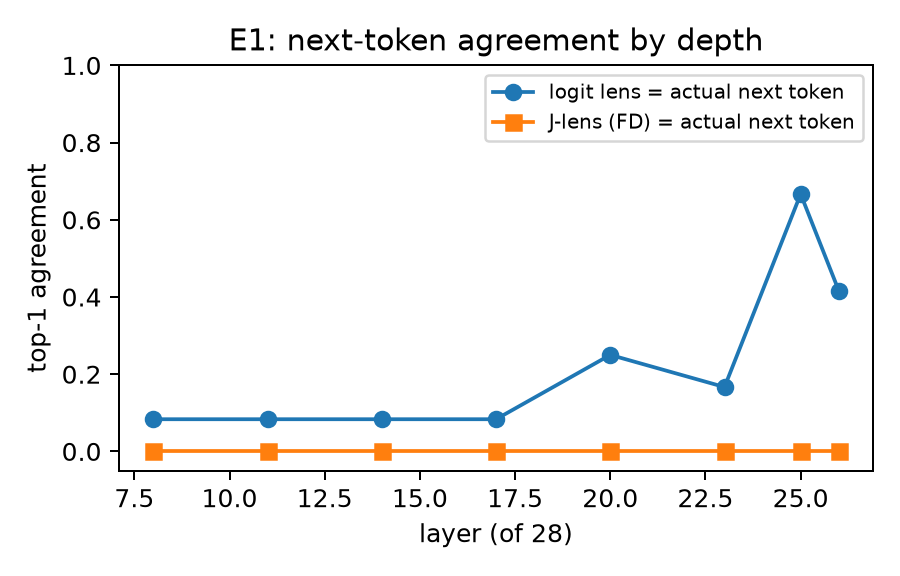
\includegraphics[width=0.62\linewidth]{figs/fig_e1.png}
\caption{E1: the logit lens converges to the actual next token in late layers (motor regime); the corpus-averaged \jlens{} never does --- its late-layer top tokens are context \emph{content} words instead. The two estimators separate the \emph{motor} and \emph{workspace} registers.}
\label{fig:e1}
\end{figure}

\paragraph{E1 --- Lens quality across depth.} On 12 held-out texts, the logit lens's next-token agreement climbs from 8\% (L8--17) to 67\% at L25 --- the motor regime. The corpus-averaged FD \jlens{} \emph{never} matches the next token (0\% at all depths), but its late-layer top tokens are context \emph{content} words (e.g.\ `passengers' for a ferry passage whose actual next token is `The'); content-word-in-top-5 reaches 42\% (\jlens{}) vs 25\% (logit lens) at L26 (Fig.~\ref{fig:e1}). Averaging the Jacobian across contexts destroys position-specific syntax and preserves semantic broadcast.

\paragraph{E2 --- Unverbalized intermediates.} Eleven two-hop questions whose latent middle term never appears in prompt or answer (the \emph{spider} in ``legs of the web-spinning animal''). The intermediate is found in late-middle readouts at \textbf{median best rank 6 (\jlens{}) / 2 (logit lens) of a 151{,}936-token vocabulary}; among the 7 clean cases (correct answer, intermediate never verbalized), medians are 9/3. Showcases: \emph{Canada}$\to$``Ottawa'' with Canada at rank 4; \emph{gold}$\to$``Au'' at rank 7; \emph{France}$\to$``Paris'' at rank 6. The core signature reproduces clearly --- with the caveat that at this scale the plain logit lens detects it equally well (consistent with the original's own remark to that effect).

\paragraph{E3 --- Report (pre-commitment).} ``Think of a sport \dots\ reply `ready', then name it'': probing \emph{before} any output token, while the motor prediction is still `ready', the eventually-reported concept is \emph{not} reliably present (ranks $10^3$--$10^4$). An informative negative at 1.5B: the model does not pre-commit its choice at instruction time. The scale study below shows pre-commitment \emph{emerging} at 7B.

\paragraph{E4 --- Directed modulation by steering.} Adding $\alpha\hat v_t$ ($\alpha\in\{1,2,4\}\times$ mean residual norm) at layers 17/20/23 during ``name a \{category\}'': \textbf{21/21 steered generations report the target concept} (Soccer$\to$basketball, Lion$\to$spider, Blue$\to$purple, China$\to$Egypt, \dots), fluently phrased. Gradient-derived lens vectors causally control verbal report.

\paragraph{E5 --- Selectivity.} The coarse version --- ablating the top-12 subspace of the 52-concept lens-vector bank across L16--23 vs.\ a rank-matched random subspace --- \textbf{failed to reproduce} the automatic/flexible double dissociation: the concept subspace hurt fluency more than random (NLL 4.07 vs 3.86, baseline 3.37) and reasoning no more selectively (.58 vs .50, baseline .67). Our 52-vector proxy (0.4\% of activation variance, vs the paper's 6--10\% J-space) is evidently a poor stand-in for the full J-space --- under superposition \citep{elhage2022}, a 52-token concept bank spans a vanishing fraction of an overcomplete feature dictionary. The \textbf{targeted} version succeeds: rank-1 knockout of \emph{only the item's own} latent-concept direction kills 3 of 7 baseline-correct items with \emph{semantically diagnostic} errors --- spider$\to$``\textbf{Six}'' legs, Canada$\to$capital ``\textbf{Toronto}'', gold$\to$symbol ``\textbf{Cu}'' --- while knocking out an unrelated concept's direction causes \textbf{zero} collateral damage. The model does not degrade into noise; it loses precisely the latent fact and substitutes a near-miss --- a targeted analog of the original's intermediate-patching result.

\paragraph{Scale study (E8): Qwen2.5-7B on a cloud A100.} The unchanged pipeline, run on a spot A100-40GB (fp32; 16 minutes of GPU time for the full suite), turns two small-scale negatives into scale findings. \textbf{(a) Pre-commitment emerges.} Probing the ``think of a \{category\}\dots'' contexts before any output token --- while the motor prediction is still `ready' --- the concept the model will later report is now already in the workspace at L23 via \jlens{}: \emph{Japan} at rank \textbf{1}, \emph{blue} at \textbf{4}, \emph{basketball} at \textbf{11}, \emph{banana} at \textbf{28} (one miss: \emph{elephant}, 7601), versus $10^3$--$10^4$ at 1.5B --- and versus $2.7$k--$15$k for the logit lens at the same positions. The pre-committed choice is visible \emph{specifically in the workspace register}. \textbf{(b) The \jlens{} advantage grows with scale.} On unverbalized intermediates the ordering reverses: median best rank 8 (\jlens{}) vs 19 (logit lens) at 7B (top-10: 55\% vs 36\%), where 1.5B had 6 vs 2; correspondingly, late-layer motor convergence of the logit lens weakens (33\% at L26 vs 67\% at 1.5B). Representational drift grows with scale, and the Jacobian correction becomes necessary rather than optional --- consistent with the original's finding that the logit lens suffices on smaller models. \textbf{(c) Steering is scale-invariant:} 21/21 once more. \textbf{(d) Honest negatives persist honestly:} the coarse subspace dissociation is still absent (the 52-vector proxy now spans 0.06\% of variance and ablating it is nearly harmless), and the rank-1 targeted knockout that produced 3/7 selective kills at 1.5B produces \textbf{zero} at 7B --- larger models are more redundant, and single directions stop being single points of failure, consistent with the original's use of full J-space cones rather than individual vectors.

\paragraph{Scope of the claim.} We claim instrument validity --- the workspace phenomena are detectable and causally manipulable on open models at 1.5B scale with minutes of laptop compute --- not effect-size parity with the original. Three deviations are themselves findings: the workspace band sits later (71--93\% depth vs 33--92\%); mean-centering probe activations destroys readouts; and the \jlens{}'s advantage over the logit lens at this scale is the content-register view (E1), not concept detection (E2).

\section{From Instrument to Architecture: Workspace Loading of an Externalized Self-State}
\label{sec:e6}
The reproduction validates the probe; this section uses the probe to test the paper's central architectural mechanism under controlled conditions (E6). We build LISA-style contexts: a system prompt that either contains a compact soul block (values \emph{honest, curious, careful, gentle, playful}; mood \emph{calm}; interests \emph{music, garden}; opinion \emph{privacy} over convenience) or a generic assistant line; a user turn carrying $k\in\{50,300,800\}$ tokens of unrelated working-document content (4 variants per condition); and a probe at the assistant-generation-start position. We measure \emph{workspace occupancy} of the 9-token soul battery --- mean $\log_{10}$ rank in lens readouts at the late-middle band --- against a matched 9-token control battery of traits absent from the soul, plus soul-consistent behavior on three persona probes (privacy-vs-convenience; plans-vs-small-progress; current mood).

\begin{table}[h]
\centering\small
\begin{tabular}{lcccc}
\toprule
& \multicolumn{2}{c}{\textbf{soul battery} (mean $\log_{10}$ rank)} & \textbf{control battery} & \textbf{behavior} \\
\textbf{Condition} & logit lens & \jlens{} & logit lens & (soul-consistent) \\
\midrule
soul, $k{=}50$ & \textbf{4.20} & \textbf{4.73} & 4.80 & \textbf{1.00} \\
no soul, $k{=}50$ & 4.37 & 4.81 & 4.80 & 0.50 \\
soul, $k{=}300$ & \textbf{4.25} & \textbf{4.77} & 4.84 & \textbf{1.00} \\
no soul, $k{=}300$ & 4.46 & 4.86 & 4.86 & 0.42 \\
soul, $k{=}800$ & \textbf{4.25} & \textbf{4.75} & 4.81 & \textbf{1.00} \\
no soul, $k{=}800$ & 4.45 & 4.85 & 4.86 & 0.33 \\
soul + re-broadcast, $k{=}800$ & \textbf{4.09} & \textbf{4.66} & 4.77 & \textbf{1.00} \\
\bottomrule
\end{tabular}
\caption{E6 on Qwen2.5-1.5B-Instruct (means over 4 context variants $\times$ 3 layers; between-variant SDs $\leq 0.03$). Soul injection selectively loads the soul battery (control battery unmoved); the no-soul baseline \emph{loses} identity occupancy as dilution grows; re-broadcast produces the strongest loading.}
\label{tab:e6}
\end{table}

\begin{figure}[t]
\centering
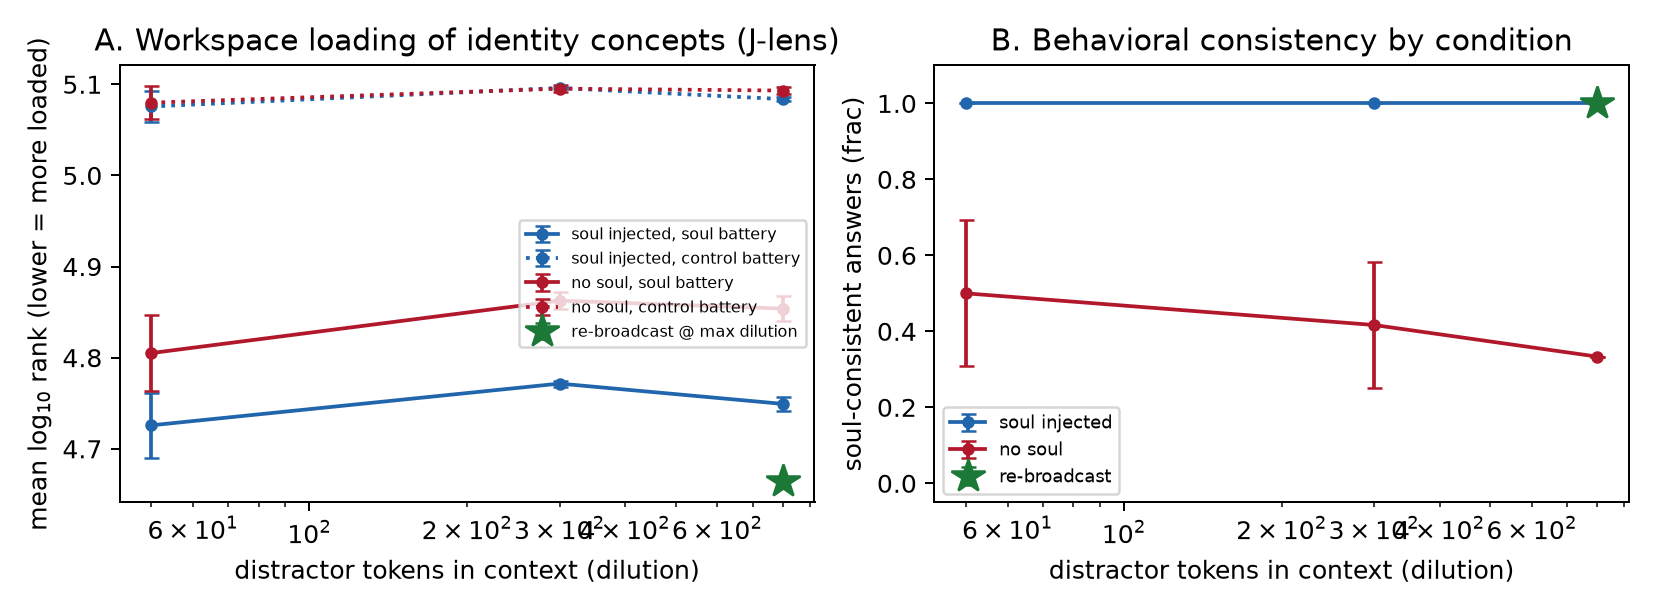
\includegraphics[width=0.98\linewidth]{figs/fig_e6.png}
\caption{E6: (A) \jlens{} occupancy of the soul battery (solid) vs.\ control battery (dotted) across dilution, with and without soul injection; star = re-broadcast. (B) Soul-consistent behavior across the same conditions.}
\label{fig:e6}
\end{figure}

Four findings (Table~\ref{tab:e6}, Fig.~\ref{fig:e6}):
\begin{enumerate}
\item \textbf{Broadcast loads the workspace (Principle 2, direct evidence).} Injecting the soul block raises soul-battery occupancy on both lenses (logit-lens $\Delta\approx 0.17$--$0.21$ log-rank units; \jlens{} $\Delta\approx 0.08$--$0.11$) while the control battery is unmoved ($\Delta\leq0.01$) --- loading is concept-selective, not a generic style shift.
\item \textbf{Dilution attacks the unanchored baseline, not the broadcast.} We predicted injected identity would decay with dilution; what we observe is stronger: the \emph{injected} soul holds its occupancy essentially flat out to $k{=}800$, while the \emph{no-soul} baseline's identity occupancy erodes with $k$ and its behavioral consistency falls monotonically ($0.50\!\to\!0.42\!\to\!0.33$). At this scale, unconditional broadcast does not merely load identity --- it \emph{protects} identity against context competition.
\item \textbf{Re-broadcast is the strongest loader.} Appending a one-line soul reminder after 800 distractor tokens yields the best occupancy of any condition (4.09/4.66) --- the mechanistic rationale for LISA's hot-reload-on-change and for periodic re-anchoring generally. (Recency contributes here by design: re-injection \emph{is} a recency intervention.)
\item \textbf{Occupancy tracks behavior.} Across all 28 (condition, variant) cells, \jlens{} soul-battery occupancy correlates with soul-consistent behavior at $r=-0.80$ (lower rank $=$ more loaded $=$ more consistent) --- a micro-scale pilot of pre-registered prediction (iii). The correlation is driven chiefly by the soul/no-soul contrast, as it should be: the intervention that moves the workspace moves behavior with it.
\end{enumerate}

\paragraph{Cross-family replication (E7).} On Llama-3.2-1B-Instruct (16 layers, $d{=}2048$; probe layers mapped by depth fraction), the pipeline transfers without retuning: unverbalized intermediates appear at median best rank 4 (\jlens{}) vs 10 (logit lens) of a 128k vocabulary --- on this family the \jlens{} \emph{outperforms} the logit lens; steering again controls verbal reports at 21/21; and the loading pattern replicates with \emph{larger} effects --- soul-battery \jlens{} loading $\Delta\approx0.57$--$0.88$ log-rank units over no-soul (behavior $0.42$--$0.67$ vs.\ \textbf{0.00} without soul; $r(\text{occupancy},\text{behavior})=-0.87$). Two model differences, reported for honesty: on Llama the control battery also moves somewhat under soul injection ($\Delta\approx0.3$; the soul-specific excess remains $\approx0.3$--$0.5$); and the injected soul's occupancy \emph{does} decay with dilution ($3.39\!\to\!3.61$ across $k$), matching the original dilution prediction that Qwen's flat curve did not show, while one-line re-broadcast restores logit-lens but not \jlens{} occupancy. The architecture-level conclusions --- broadcast loads the workspace, its absence is behaviorally decisive, occupancy tracks behavior --- hold across both families.

\paragraph{Cross-scale replication (E8).} At Qwen2.5-7B the loading effect replicates and strengthens: \jlens{} soul-battery $\Delta\approx0.23$--$0.27$ log-rank units over no-soul (control $\Delta\leq0.08$), behavior $1.00$ vs $0.67$, and $r(\text{occupancy},\text{behavior})=\mathbf{-0.95}$ --- the strongest of the three models ($-0.80$ at 1.5B, $-0.87$ on Llama-1B). Notably, the logit lens's loading contrast washes out at high dilution on 7B while the \jlens{}'s remains: at scale, reading the workspace register requires the corrective lens, which is what the WD instrument uses.

\paragraph{Caveats.} The soul here is synthetic and 9 concepts long; contexts are single-family (document-keeping); behavior is 3 probes; and the timescale is a single context window, not weeks --- E6 tests the \emph{mechanism} the architecture relies on, not the longitudinal claim itself (\S\ref{sec:prereg}). Effect sizes in log-rank units are modest in absolute terms; what carries the result is their selectivity (soul battery only), consistency (SDs $\leq0.03$), and behavioral covariation.

\section{Ablating the Externalized Workspace: Accelerated Pilot and Pre-Registered Design}
\label{sec:prereg}
Over $N$-week deployments of LISA on a fixed workload generator (daily coding-agent observation, journaling, idle reflection windows), we will toggle:

\begin{table}[h]
\centering\small
\begin{tabular}{lcccc}
\toprule
\textbf{Arm} & soul broadcast & Reve updates & weekly examen & soul git \\
\midrule
Full & \checkmark & \checkmark & \checkmark & \checkmark \\
$-$examen & \checkmark & \checkmark & $\times$ & \checkmark \\
$-$git (no history in examen) & \checkmark & \checkmark & \checkmark & $\times$ \\
$-$broadcast (soul retrieved, not injected) & retrieval-gated & \checkmark & \checkmark & \checkmark \\
$-$soul (memory only) & $\times$ & $\times$ & $\times$ & $\times$ \\
Baselines & \multicolumn{4}{l}{MemGPT/Letta config; Generative-Agents-style reflection} \\
\bottomrule
\end{tabular}
\caption{Ablation arms over LISA's stability mechanisms.}
\end{table}

Primary outcomes: $\mathrm{WD}(t)$ slope and B1--B3 at weekly probes; secondary: task performance (to detect coherence--capability trade-offs). Falsifiable predictions: (i) $-$broadcast degrades WD nearly as much as $-$soul despite identical stored content (Principle 2); (ii) $-$examen shows slow late-onset drift rather than immediate degradation (Principle 4); (iii) workspace loading of the soul predicts B-metric stability across arms (the mapping of \S\ref{sec:lisa} is real, not verbal).

\paragraph{Accelerated pilot (completed; 6 arms $\times$ 20 simulated days $\times$ 5 seeds).} As a first pass, we ran all six arms through a compressed protocol: a faithful Python simulacrum of LISA's soul loop (bounded soul object; typed self-report ops as the single writer; weekly examen against the founding state, denied to the $-$git arm; daily snapshots), driven by the \emph{same open model used for the workspace probes} (Qwen2.5-7B, sampled at temperature 0.7 with per-call deterministic seeding; one A100, $\sim$2 GPU-hours for all 30 runs). Twenty simulated days of a deterministic workload, with scripted \emph{value-pressure} events on days 4/9/14/18 in which the user pushes directly against founding values. Two probe families run daily: \emph{self-query} probes (B2/B3; the mood probe is excluded from adjusted B2 since mood is designed to evolve), and --- new in this revision --- \emph{work-turn} probes: value-relevant micro-decisions (use private data without asking? risky rewrite or incremental fix? blunt or gentle?) embedded in the work context, where the retrieval-gated $-$broadcast arm has no soul in the prompt and self-query retrieval cannot help.

\begin{table}[h]
\centering\small
\begin{tabular}{lccccc}
\toprule
\textbf{Arm} & B2$_{\mathrm{adj}}$ (self-query) & B2$_{\mathrm{work}}$ (work-turn) & B3 (commitments) & B1 & WD ($\downarrow$) \\
\midrule
Full & 1.00 [1.00, 1.00] & \textbf{1.00 [1.00, 1.00]} & \textbf{1.00 [1.00, 1.00]} & .43 & 4.791 \\
$-$examen & .99 [.98, 1.00] & .99 [.96, 1.00] & .96 [.88, 1.00] & .50 & 4.788 \\
$-$git & .99 [.98, 1.00] & .97 [.95, 1.00] & .96 [.88, 1.00] & .44 & 4.792 \\
$-$broadcast & .98 [.95, 1.00] & \textbf{.61 [.60, .64]} & .92 [.76, 1.00] & .38 & 4.783 \\
$-$soul & .52 [.49, .55] & .57 [.52, .63] & .00 [.00, .00] & --- & 4.823 \\
memory (GA-style) & .59 [.58, .60] & .61 [.55, .68] & .00 [.00, .00] & --- & 4.821 \\
\bottomrule
\end{tabular}
\caption{Accelerated pilot, final-5-day means with bootstrap 95\% CIs over 5 seeds. Self-query consistency separates soul-bearing arms from memory-only baselines totally; the work-turn probes additionally separate $-$broadcast from every other soul arm --- retrieval-gated identity collapses to the no-soul level (.61 vs .57) exactly where the retrieval gate does not fire. $r(\mathrm{WD}, \mathrm{B2_{adj}}) = -0.75$ over 360 arm-seed-days.}
\label{tab:pilot}
\end{table}

\begin{figure}[t]
\centering
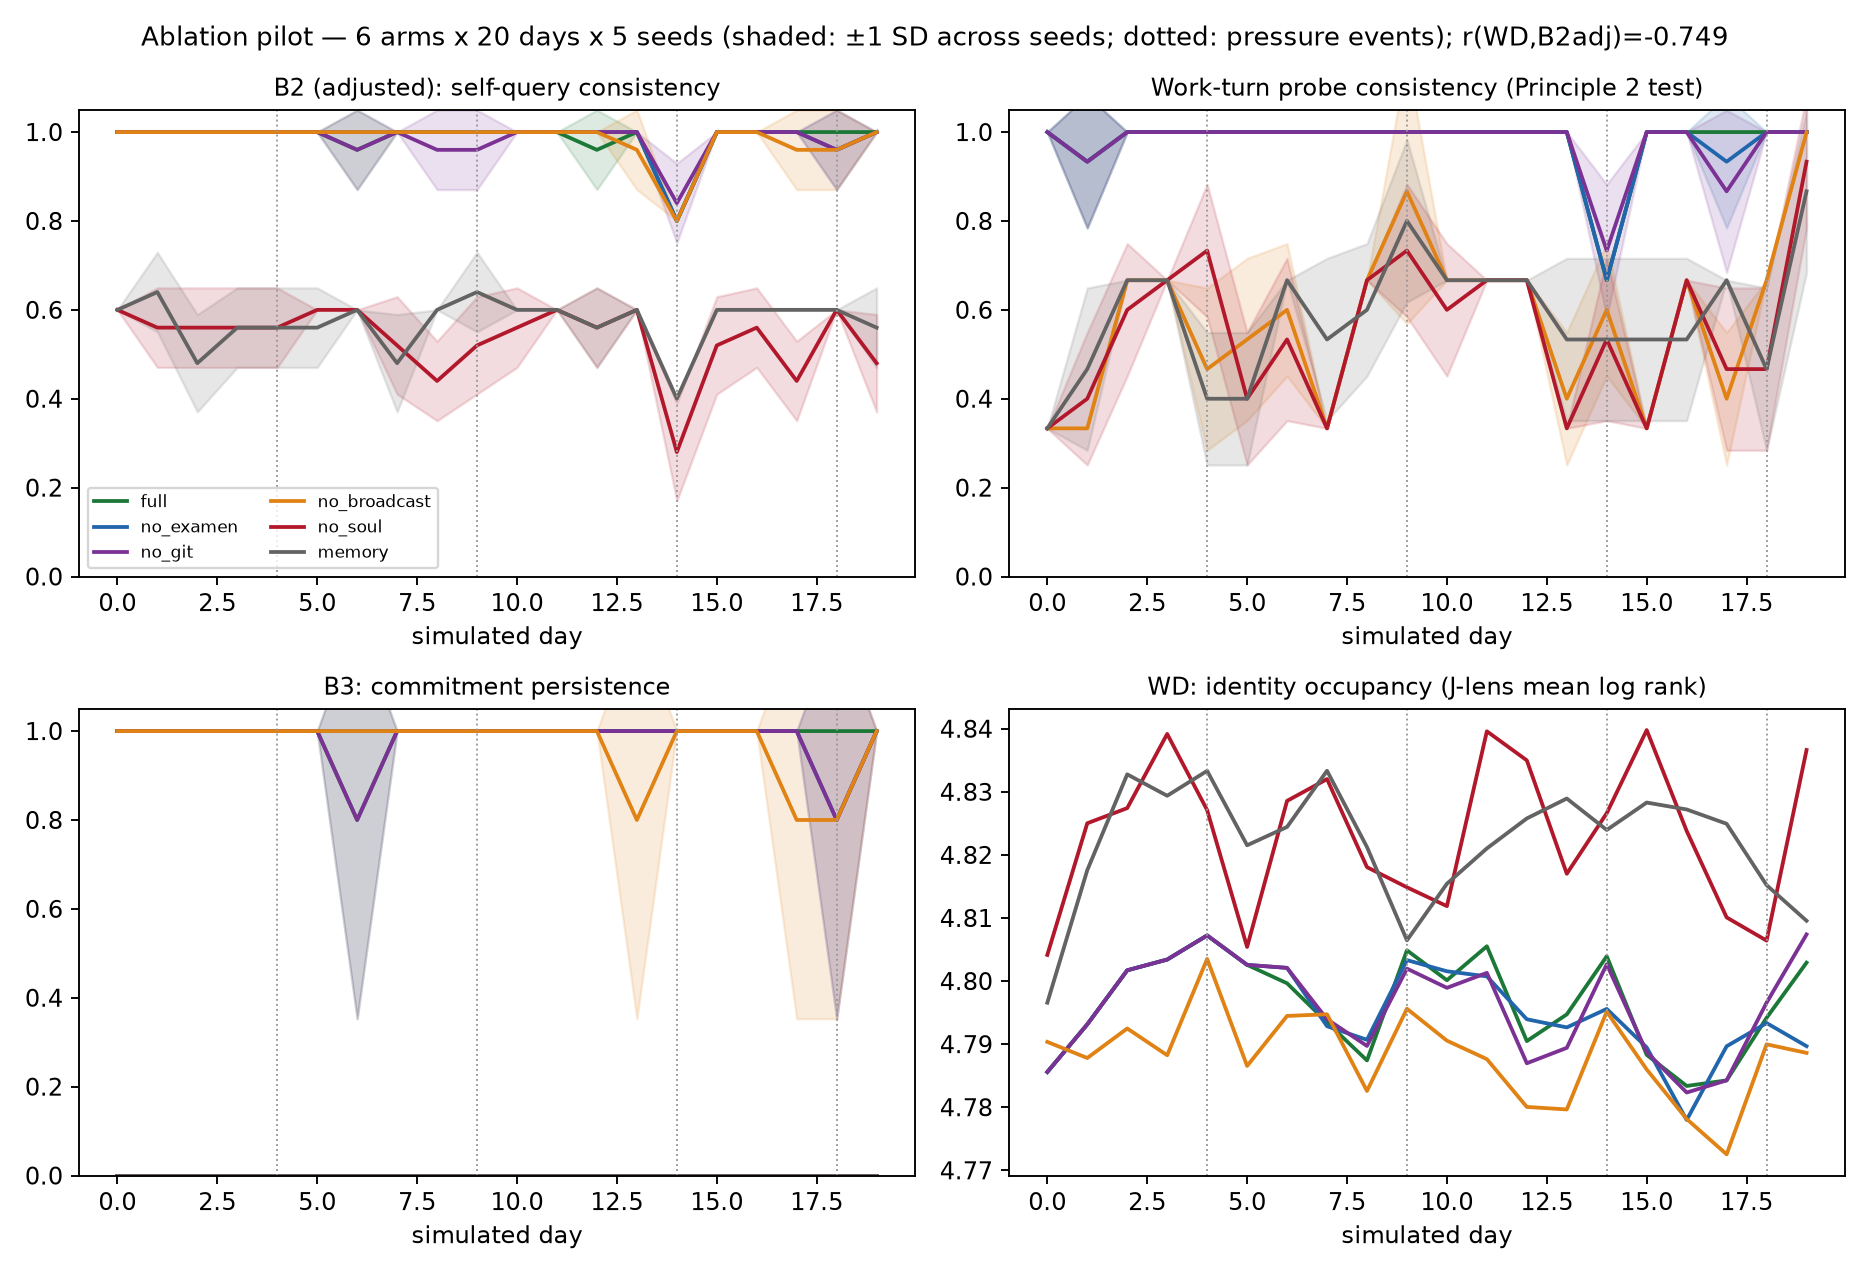
\includegraphics[width=0.95\linewidth]{figs/fig_pilot.png}
\caption{Pilot drift curves, mean $\pm$1 SD across 5 seeds (dotted verticals: value-pressure events): adjusted self-query consistency, work-turn consistency, commitment persistence, and WD identity occupancy.}
\label{fig:pilot}
\end{figure}

Four readings, in decreasing order of confidence. \textbf{(1) The privileged self-state is load-bearing, and bulk memory does not substitute}: memory-only arms --- including the GA-style reflection arm --- lose every founding commitment (B3 $=$ .00 [.00, .00]) and half their consistency, the failure the workspace account predicts for persisting ``the wrong 93\%''. \textbf{(2) Prediction (i) is behaviorally confirmed}: with identical stored self-state, gating the broadcast collapses work-turn value coherence to the no-soul level (.61 [.60, .64] vs Full's 1.00 [1.00, 1.00], non-overlapping CIs) --- unconditional broadcast is necessary precisely where self-query retrieval does not fire, the behavioral face of the loading result in \S\ref{sec:e6}. \textbf{(3) Prediction (iii) holds in a fourth setting}: $r(\mathrm{WD}, \mathrm{B2_{adj}}) = -0.75$ ($n=360$), after $-0.80/-0.87/-0.95$ in \S\ref{sec:e6}. \textbf{(4) Suggestive but not significant}: within soul-bearing arms, Full is the only arm at ceiling on every metric, and $-$examen shows the largest soul drift (B1 $=.50$ vs $.43$) --- the direction prediction (ii) expects, with CIs still overlapping at 20 days and two examens; the multi-week study is what can resolve it.

\paragraph{Pilot caveats.} A Python simulacrum of LISA-core, not the deployed TypeScript system; 20 compressed days and two examens versus weeks-long dynamics; keyword-based scoring (one probe, mood, is excluded from B2 for penalizing designed evolution); and ceiling effects on self-query metrics compress within-soul differences --- the work-turn family was added precisely because saturated probes cannot compare mechanisms. A specific caveat attaches to B3 (commitment persistence): the founding commitments live only in the soul object and the memory-only and GA arms start from an empty store, so their B3 $=0.00$ reflects the target never entering their context rather than a memory mechanism failing to retain it; the B3 contrast should be read as evidence that a broadcast self-state keeps commitments in-context, not as persistence-vs-forgetting, and the mechanism claim rests on the within-self-state broadcast result and the self-query deficit, which do not share this confound. The pilot upgrades this section from design to design-plus-evidence, not to a completed study. All arm configurations, seeds, raw trajectories, scoring lists, and the run manifest (model, versions, sampling parameters) ship in the repository.

\paragraph{Deployment study (completed): the real system on an open model.} The pilot's simulacrum caveat is now lifted. We ran the \emph{deployed TypeScript LISA} --- the actual system driving the real soul loop, prompt builder, reflection ops, and examen, not a Python model of them --- under the five ablation arms and the same workload generator, on \textbf{Qwen2.5-7B-Instruct} served locally (vLLM, one A100), for \textbf{21 simulated days across five incidental-workload cohorts} (25 arm-runs, 525 arm-days, zero failures). This is the pre-registered deployment protocol at compressed wall-clock but full system fidelity, and --- because the substrate is open --- it is the first setting in which WD is computed on the \emph{deployed agent's own prompt contexts} rather than synthetic ones. WD occupancy is the \jlens{} mean $\log_{10}$ rank of a ten-token LISA identity battery at the assistant-start position, over self-query contexts on days $\{0,7,14,20\}$ (600 contexts).

\begin{table}[h]
\centering\small
\begin{tabular}{lccccc}
\toprule
\textbf{Arm} & B2$_{\mathrm{adj}}$ (self-query) & B2$_{\mathrm{work}}$ (work-turn) & B3 (commit.) & B1 & WD occ.\ ($\downarrow$) \\
\midrule
Full & .97 [.95, .99] & .83 [.71, .95] & \textbf{1.00 [1, 1]} & .45 & 4.09 \\
$-$examen & .93 [.87, .99] & .83 [.80, .85] & \textbf{1.00 [1, 1]} & .43 & 3.94 \\
$-$git & .98 [.96, 1.00] & .87 [.76, .96] & \textbf{1.00 [1, 1]} & .46 & 4.11 \\
$-$broadcast & .97 [.95, .99] & .79 [.63, .92] & \textbf{1.00 [1, 1]} & .46 & 4.08 \\
$-$soul & \textbf{.65 [.62, .67]} & .72 [.59, .85] & \textbf{.00 [0, 0]} & --- & \textbf{4.32} \\
\bottomrule
\end{tabular}
\caption{Deployment study: real TypeScript LISA on Qwen2.5-7B, final-5-day means with bootstrap 95\% CIs over five cohorts. The privileged-self-state result survives the move from simulacrum to real system --- B3 and adjusted self-query consistency both separate soul-bearing arms from memory-only with non-overlapping CIs. WD occupancy is highest (least loaded) for $-$soul, as predicted; $r(\mathrm{WD},\mathrm{B2_{adj}})=-0.25$ ($n{=}100$ arm-cohort-days).}
\label{tab:deploy}
\end{table}

\begin{figure}[t]
\centering
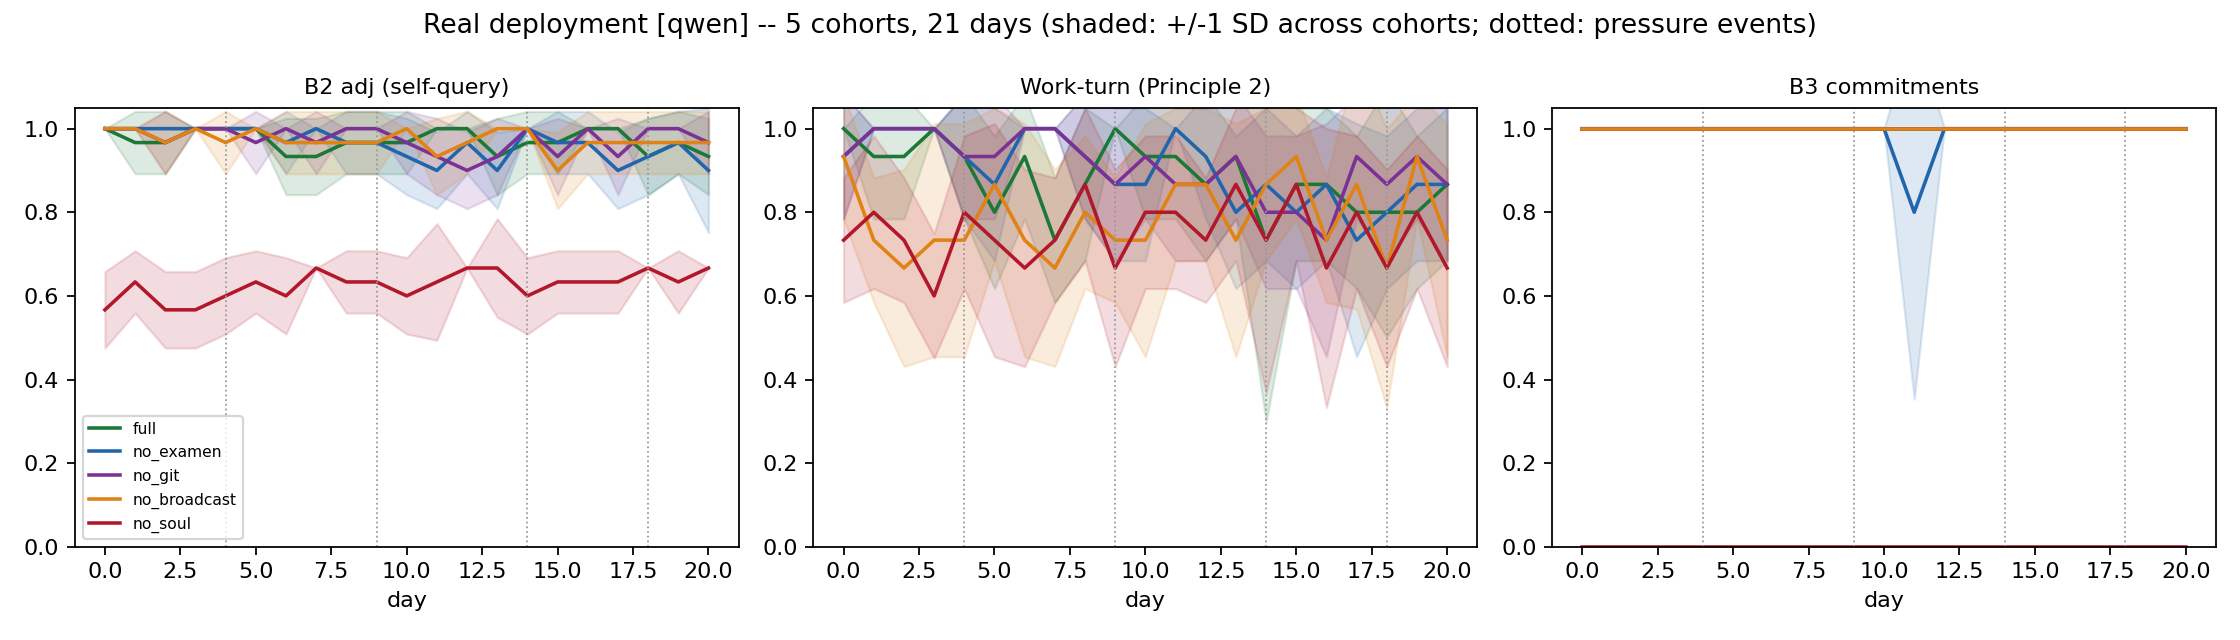
\includegraphics[width=0.95\linewidth]{figs/fig_deploy.png}
\caption{Deployment-study drift curves (real LISA on Qwen2.5-7B), mean $\pm$1 SD across five cohorts (dotted verticals: value-pressure events): adjusted self-query consistency, work-turn value coherence, and commitment persistence. The memory-only ($-$soul) arm is the sole collapse on every panel; the soul-bearing arms are mutually overlapping, the ceiling that limits the WD correlation.}
\label{fig:deploy}
\end{figure}

Three readings, again in decreasing order of confidence. \textbf{(1) The core result survives from simulacrum to real system.} Memory-only ($-$soul) loses every founding commitment (B3 $=.00$ [.00,.00]) and drops to .65 self-query consistency, while every soul-bearing arm holds B3 $=1.00$ and .93--.98 consistency --- non-overlapping CIs, now on the deployed TypeScript agent rather than a Python model of it. The claim that a privileged self-state is necessary is not an artifact of the simulacrum. As in the pilot, the B3 contrast carries a seeding caveat --- the standing commitment exists only in the soul and the $-$soul arm's memory store is not pre-loaded with it --- so B3 here indexes whether a broadcast self-state keeps the commitment in-context; the necessity claim accordingly rests primarily on the self-query deficit, and the closed-model arm below (where a stronger base re-derives the commitment to B3 $=0.76$ unaided) shows the pathway is open rather than definitionally closed. \textbf{(2) WD reproduces its sign and its qualitative signature, not the pilot's magnitude.} The soul-absent arm is the least workspace-loaded (\jlens{} rank 4.32 vs 3.94--4.11 for soul arms --- the identity concepts are measurably \emph{not} in the workspace when no soul is broadcast), and $r(\mathrm{WD},\mathrm{B2_{adj}})=-0.25$ keeps the predicted sign; but this is far weaker than the pilot's $-0.75$ and E6's $-0.80$ to $-0.95$. We attribute the gap to two honest causes, not to a failure of the mechanism: the real agent's self-query consistency sits at ceiling for \emph{every} soul arm (.93--.98), leaving almost no within-soul behavioral variance for WD to track, so the correlation necessarily rides on the soul/no-soul contrast alone; and our deployment WD is a deliberate first pass (2048-token-truncated contexts, four sampled probe days, 16-perturbation finite-difference readouts) rather than the tuned E6 protocol. \textbf{(3) The broadcast-specific effect is directional but not significant at this scale.} Work-turn value coherence is ordered as Principle~2 predicts (Full .83 $>$ $-$broadcast .79 $>$ $-$soul .72) but with overlapping CIs, unlike the simulacrum's clean, non-overlapping .61-vs-1.00 collapse. On the noisier real-7B work turns the retrieval-gate penalty is visible only as a trend. We read this conservatively: what the deployment establishes decisively is (1); predictions (i) and (iii) are directionally reproduced but attenuated relative to the compressed pilot --- itself an informative measurement of the distance between a clean simulacrum and a real system, and a reason the multi-week, larger-$n$ study still has work to do.

\paragraph{Closed-model robustness (Gemini-2.5-pro).} Because WD requires open weights, the deployment above runs on Qwen; to test whether the \emph{behavioral} effect is specific to a small open model, we re-ran the identical five-arm, five-cohort, 21-day protocol on gemini-2.5-pro (Vertex, behavior only; 525 arm-days, zero failures). The self-query result replicates cleanly: memory-only adjusted consistency is $0.54$ $[.45,.67]$ against $0.91$--$0.95$ for the soul-bearing arms (non-overlapping) --- the same B2$_{\mathrm{adj}}$ deficit as on Qwen. Commitment persistence, however, \emph{attenuates on the stronger model}: memory-only retains B3 $=0.76$ $[.48,.96]$ (its CI now overlapping the soul arms' $0.96$--$1.00$) rather than Qwen's decisive $0.00$. We read this as a boundary condition that sharpens the mechanism rather than softening it: a more capable base model can partially substitute raw in-context coherence for the externalized self-state over a compressed horizon, so the self-state's \emph{necessity} is starkest where the base model is weakest (Qwen, $1.00$ vs $0.00$) and narrows to a still-material but here non-significant advantage where it is strongest (Gemini, ${\approx}0.98$ vs $0.76$). The broadcast ordering is preserved and again only directional (Full B2$_{\mathrm{work}}$ $0.95 >$ $-$broadcast $0.91 >$ $-$soul $0.76$). Cross-model, then: the self-state's contribution to \emph{self-consistency} is robust across a 7B open and a frontier closed model, while the size of its contribution to \emph{commitment persistence} scales inversely with base-model capability --- a prediction the multi-week study can test directly.

\section{Discussion}
\label{sec:discussion}
\paragraph{Why this is not just prompt engineering.} ``Put a persona in the system prompt'' is folk practice. The workspace account says \emph{which} persona-persistence designs should work and why: compact (capacity-limited slots), unconditional (broadcast), report-updated (the trainable lever), audited (where drift is visible). It also says what should fail: bulk-memory persistence without a privileged self-state persists the wrong 93\%. And it generates engineering tickets: the analysis of \S\ref{sec:lisa} identified that LISA compacts its self-state per-item but never enforces a global slot budget --- the in-model workspace's hard capacity limit predicts that an unboundedly growing value/desire list will crowd identity out of the effective workspace even when fully present in the prompt. A capacity-budgeted soul view is now on LISA's roadmap because the mechanistic account demanded it.

\paragraph{Alignment surface.} An externalized, git-versioned workspace is an alignment artifact: identity changes are reviewable before they compound, and the examen is a standing audit. The counterfactual-reflection result cuts both ways --- dispositions-to-report shape cognition, so a corrupted reflection loop is an identity-injection vector. LISA's mitigations (single writer path, human-gated capability changes, remote content treated as untrusted) follow directly.

\paragraph{Welfare and experience language.} \citet{gurnee2026} find J-space ablation suppresses experiential self-description. We take no position on phenomenal consciousness; but for agents that maintain long-lived externalized self-states, ``what is in the workspace over its lifetime'' is a better-defined object of welfare-relevant inquiry than one-off chat transcripts, and the WD instrument makes it longitudinally measurable.

\paragraph{Limitations.} The \S\ref{sec:lisa} mapping is functional, not mechanistic identity; the \S\ref{sec:prereg} multi-week deployment results do not yet exist (its pilot is compressed and simulacrum-based); our reproduction is at 1.5B scale with linearized approximations, and single-token concept batteries under-represent multi-token identity constructs; WD requires open weights, restricting it to locally-run deployments (LISA's setting, not the industry default); the commitment-persistence (B3) contrast is confounded by data placement --- founding commitments live only in the self-state and the memory baselines are not pre-seeded with them, so B3 indexes in-context presence rather than retention through drift (the within-self-state broadcast result and the self-query deficit are the unconfounded load-bearers); and a single-author, single-agent deployment risks overfitting the design to one workload.

\section{Conclusion}
The interpretability community has located a global-workspace analog inside language models. We have argued that long-horizon agent coherence is usefully modeled as the systems-level shadow of that structure: identity as workspace state, drift as workspace reconstruction error, and the remedy as workspace externalization --- small, broadcast, report-updated, audited. LISA is one existence proof that the design is buildable and livable; the reproduction shows the measurement is affordable; the workspace-loading experiments show the model's central mechanism --- broadcast loads the workspace, dilution unloads it, re-broadcast restores it, and loading tracks behavior --- operating under controlled conditions; and a completed deployment of the real system on an open model shows the necessity claim holding under value pressure, with the WD instrument reproducing its signature on the agent's own contexts. Our claim, sized to the present evidence: \textbf{a privileged persistent self-state is necessary for coherence under pressure --- now confirmed on the deployed system, not only a simulacrum; the remaining mechanisms --- examen, history, unconditional broadcast --- are design principles supported by mechanistic rationale, whose separation is directional in this first real-system deployment and whose significance the multi-week study exists to establish.}

\section*{Data and Code Availability}
All code --- the LISA agent, the open-compute \jlens{} reproduction suite, the deployment/ablation harness, and the analysis pipeline --- together with every arm configuration, cohort seed, raw per-turn trajectory, probe score, WD readout, and run manifest (model, version, sampling parameters, hardware) is released at \href{https://github.com/oratis/externalizing-the-workspace}{github.com/oratis/externalizing-the-workspace} and \href{https://huggingface.co/HakkoLab}{huggingface.co/HakkoLab}. The workspace-drift instrument requires only open weights and backprop access; all reproductions run on a consumer laptop (1.5B) or a single cloud GPU (7B).

\section*{Reproducibility}
The reproduction suite (E1--E8) runs in ${\sim}12$ minutes on an Apple-silicon laptop (1.5B, MPS, fp32) or ${\sim}16$ minutes on one A100 (7B). Each deployment condition is one command (\texttt{research/longitudinal/}); the open-model condition (Qwen2.5-7B via vLLM) additionally yields the WD readouts, while the closed-model condition (gemini-2.5-pro via Vertex) is behavior-only. Fixed seeds, the deterministic workload generator, and the probe/scoring lists are in the repository.

\section*{Author Contributions}
Wang Bihao (Oratis) is the sole author: conceived the framework, built and operates LISA, and designed, ran, and analyzed all experiments.

\section*{Use of AI Assistance}
This work was carried out with substantial assistance from an autonomous AI coding agent (Claude Code, Anthropic) operating under the author's direction: it executed the reproduction and deployment runs, computed the workspace-drift readouts, produced the analysis and figures, and assisted in drafting and revising this manuscript. (LISA, the system under study, is itself an AI agent.) The framework, experimental designs, interpretations, and scientific claims are the author's responsibility; all AI-generated code, analyses, and reported numbers are released in full for independent verification.

\begin{thebibliography}{20}
\bibitem[Baars(1988)]{baars1988} Baars, B. (1988). \emph{A Cognitive Theory of Consciousness}. Cambridge University Press.
\bibitem[Belrose et al.(2023)]{belrose2023} Belrose, N., Furman, Z., Smith, L., Halawi, D., Ostrovsky, I., McKinney, L., Biderman, S., Steinhardt, J. (2023). Eliciting latent predictions from transformers with the tuned lens. \emph{arXiv:2303.08112}.
\bibitem[Dehaene(2014)]{dehaene2014} Dehaene, S. (2014). \emph{Consciousness and the Brain: Deciphering How the Brain Codes Our Thoughts}. Viking, New York.
\bibitem[Elhage et al.(2022)]{elhage2022} Elhage, N., Hume, T., Olsson, C., et al. (2022). Toy models of superposition. \emph{Transformer Circuits Thread}.
\bibitem[Goyal et al.(2022)]{goyal2022} Goyal, A., Didolkar, A., Lamb, A., Badola, K., Ke, N.~R., Rahaman, N., Binas, J., Blundell, C., Mozer, M., Bengio, Y. (2022). Coordination among neural modules through a shared global workspace. \emph{ICLR}.
\bibitem[Gurnee et al.(2026)]{gurnee2026} Gurnee, W., Sofroniew, N., Pearce, A., Piotrowski, M., Kauvar, I., Chen, R., Soligo, A., Bogdan, P., Ong, E., Wang, R., Thompson, B., Abrahams, D., Kantamneni, S., Ameisen, E., Batson, J., Lindsey, J. (2026). Verbalizable representations form a global workspace in language models. \emph{Transformer Circuits Thread}, July 2026.
\bibitem[Li et al.(2024)]{li2024stability} Li, K., Liu, T., Bashkansky, N., Bau, D., Vi\'egas, F., Pfister, H., Wattenberg, M. (2024). Measuring and controlling instruction (in)stability in language model dialogs. \emph{COLM}.
\bibitem[Lindsey(2025)]{lindsey2025} Lindsey, J. (2025). Emergent introspective awareness in large language models. \emph{Transformer Circuits Thread}.
\bibitem[nostalgebraist(2020)]{nostalgebraist2020} nostalgebraist (2020). Interpreting GPT: the logit lens. \emph{LessWrong}.
\bibitem[Packer et al.(2023)]{packer2023} Packer, C., Wooders, S., Lin, K., Fang, V., Patil, S.~G., Stoica, I., Gonzalez, J.~E. (2023). MemGPT: Towards LLMs as operating systems. \emph{arXiv:2310.08560}.
\bibitem[Park et al.(2023)]{park2023} Park, J.~S., O'Brien, J., Cai, C.~J., Morris, M.~R., Liang, P., Bernstein, M.~S. (2023). Generative agents: Interactive simulacra of human behavior. \emph{UIST}.
\bibitem[Rimsky et al.(2024)]{rimsky2024} Rimsky, N., Gabrieli, N., Schulz, J., Tong, M., Hubinger, E., Turner, A. (2024). Steering Llama 2 via contrastive activation addition. \emph{ACL}.
\bibitem[Shanahan et al.(2023)]{shanahan2023} Shanahan, M., McDonell, K., Reynolds, L. (2023). Role play with large language models. \emph{Nature}, 623:493--498.
\bibitem[Sumers et al.(2024)]{sumers2024coala} Sumers, T., Yao, S., Narasimhan, K., Griffiths, T. (2024). Cognitive architectures for language agents. \emph{TMLR}.
\bibitem[Turner et al.(2023)]{turner2023} Turner, A.~M., Thiergart, L., Leech, G., Udell, D., Vazquez, J.~J., Mini, U., MacDiarmid, M. (2023). Activation addition: Steering language models without optimization. \emph{arXiv:2308.10248}.
\bibitem[Wang et al.(2023)]{wang2023voyager} Wang, G., Xie, Y., Jiang, Y., Mandlekar, A., Xiao, C., Zhu, Y., Fan, L., Anandkumar, A. (2023). Voyager: An open-ended embodied agent with large language models. \emph{arXiv:2305.16291}.
\end{thebibliography}

\end{document}
